\documentclass[conference]{IEEEtran}
\IEEEoverridecommandlockouts

\usepackage[L7x,T1]{fontenc}
\usepackage[utf8]{inputenc}
\usepackage[english, lithuanian]{babel}

% The preceding line is only needed to identify funding in the first footnote. If that is unneeded, please comment it out.
\usepackage{cite}
\usepackage{amsmath,amssymb,amsfonts}
\usepackage{algorithmic}
\usepackage{graphicx}
\usepackage{textcomp}
\usepackage{xcolor}
\usepackage{biblatex}
\bibliography{saltiniai.bib}

\def\BibTeX{{\rm B\kern-.05em{\sc i\kern-.025em b}\kern-.08em
    T\kern-.1667em\lower.7ex\hbox{E}\kern-.125emX}}

\usepackage[labelsep=endash]{caption}
\renewcommand{\figurename}{pav}

\usepackage{lipsum}

\begin{document}

\title{Rašytinės LT kalbos identifikavimas (OCR)}

\author{\IEEEauthorblockN{Paulius Milmantas}
\IEEEauthorblockA{\textit{Vilniaus universitetas} \\
\textit{Matematikos ir informatikos fakultetas}\\
Vilnius, Lietuva \\
paulius.milmantas@mif.stud.vu.lt}
}

\maketitle

\begin{abstract}
Darbe buvo spręsta rašytinės lietuvių kalbos raidžių atpažinimo problema.
Parašyta programa gali aptikti 6 išmoktas raides: A, a, B, C, P, u vidutiniškai su
85\% atspėjimo tikimybe. Padarytą sistemą galima plėsti nemodifikuojant esamo kodo:
užtenka sukurti naują duomenų rinkinį pagal tam tikrą formatą ir ištreniruoti naują
3 elementų aptikimo tinklą. Kadangi programoje naudojama daug skirtingų tinklų ir kiekvienas
jų atskiria tik 3 elementus, plečiant programą, nebereikia apmokyti visos sistemos iš naujo,
užtenka tik pridėti naują tinklą, programa jį automatiškai aptinka ir pradeda naudoti.
Naujam 3 raidžių poaibiui apmokyti reikia vidutiniškai 50 nuotraukų kiekvienai raidei ir
norint pasiekti 85\% tikslumą vidutiniškai užtenka 300 epochų. Naudojant Google Colab
platformą tai vidutiniškai užtrunka apie 10 minučių. Naudojant daug neuroninių tinklų
taip pat išspręsta didelio RAM naudojimo problema: pagal esamus resursus galima
apskaičiuoti kiek vienu momentu galima pakrauti tinklų ir pakrauti tik tam tikrą jų
kiekį.
\end{abstract}

\section{Įvadas}
Užduoties tikslas: parašyti sprendimą, kuris iš duotos
nuotraukos išgautų joje pateiktą Lietuvišką rašytinį tekstą.
Atpažinimui buvo naudojamas stochastinis gradientų nuolydis (SGD).
Buvo bandyta jį lyginti su naujai išėjusiu SGD modifikuotu variantu (pav. ~\ref{fig1}). Šio algoritmo nebuvo spėta pilnai realizuoti.

\section{Metodai}

\subsection{Taikyta nuostolių funkcija}

Darbe buvo naudota MSE (Mean Square Error) funkcija. ~\eqref{eq:lygtis1}

\begin{equation}
MSE = \frac{1}{n} \cdot \sum_{i=1}^{n} (y_{i} - y_{i}^{p})^{2}
\label{eq:lygtis1}
\end{equation}

\subsection{Optimizavimo funkcija}

Optimizavimui buvo naudota stochastinio gradientų nuolydžio
(SGD) optimizavimo funkcija ~\eqref{eq:lygtis2}. Taip pat buvo bandyta realizuoti modifikuotą SGD algoritmą (pav. ~\ref{fig1}).

\begin{equation}
\theta^{(\tau)} = \theta^{(\tau - 1)} - \eta \cdot \bigtriangledown_{\theta} Loss(\theta^{(\tau - 1)};(x_{i}, y_{i}))
\label{eq:lygtis2}
\end{equation}

\begin{figure}[!h] % įterpti čia
\centerline{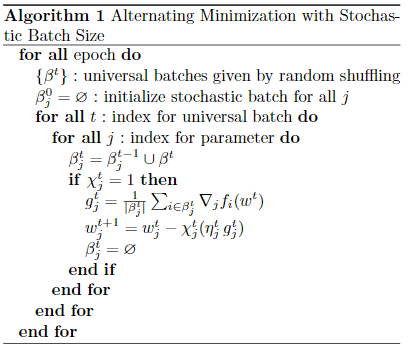
\includegraphics[scale=0.4] {images/2.png}}
\caption{SGD modifikuotas algoritmas.}
\label{fig4}
\end{figure}

\subsection{Naudojamas tinklas}

Visos abėcėlės raidės yra skirstomos į poaibius po 3 raides. Tai parodyta pav. ~\ref{fig1} Kiekvienam poaibiui yra
sukuriama po atskirą neuroninį tinklą. Taip yra lengviau atlikti tinklo treniravimą
ir tinklo užkrovimui galima sutaupyti RAM atminties. Norint pridėti daugiau
duomenų, užtenka tinklą apmokyti tik vienam naujam poaibiui.
\par
Tinklą sudaro 2 paslėpti sluoksniai, 1 įvesties ir 1 išvesties sluoksnis. Duomenys
yra 64x64 dydžio pilki vaizdai, todėl įvesties sluoksnis yra 4096 dydžio. Išvesties
sluoksnis yra 3 dydžio, nes visi poaibiai yra sudaryti iš 3 narių. Visi sluoksniai naudoja
RELU aktyvacijos funkcijas.

\begin{figure}[!h] % įterpti čia
\centerline{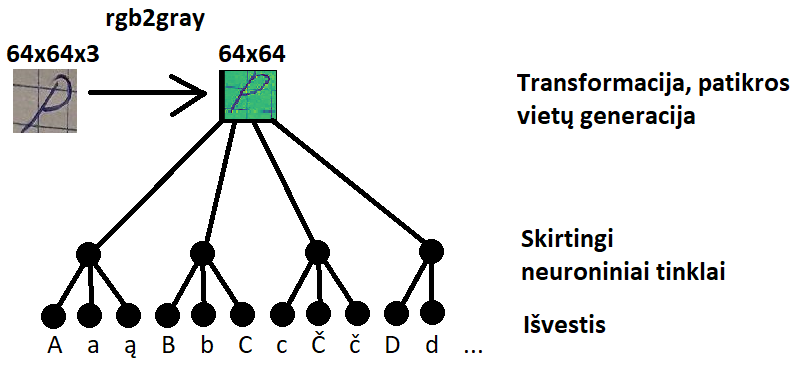
\includegraphics[scale=0.4] {images/1.png}}
\caption{Tinklo sudėtis.}
\label{fig1}
\end{figure}

\subsection{Apdorojimo sričių paieška}

% https://ieeexplore.ieee.org/abstract/document/5540041?casa_token=Mimlm6xdnKEAAAAA:uZwMcxc1uBssvCtGad4B6L8NQTub-lULk31J7ED1vkmswWcodt-Sal7ea_U4x0uDqXax0HssGAQ

Sričių radimui, kurias norima leisti per neuroninius tinklus, buvo naudojama
objektų kraštinių paieška. Kadangi kiekvieną pikselį apibrėžia tik vienas skaičius:
pilkos spalvos stiprumas, galima eiti pro paveiksliuko kiekvieną pikselį ir
tikrinti ar jo reikšmė labai skiriasi nuo praeitos. Šiuo metodu gaunamos visos kraštinės,
tačiau atsiranda ir daug triukšmo. Jis paprastai aiškiuose vaizduose būna nedidelis, todėl
jį galima pašalinti tikrinant kraštinių vientisumas: jeigu pikselis yra aptiktas kaip kraštinė,
tai jį turi supti dar nors vienas pikselis, kuris yra laikomas kraštine. Jeigu tokio pikselio šalia nėra,
reiškia tikrinamas pikselis nėra kraštinė ir jo nereikia įtraukti. Rezultatas pateiktas pav.~\ref{fig3}.

\begin{figure}[!h] % įterpti čia
\centerline{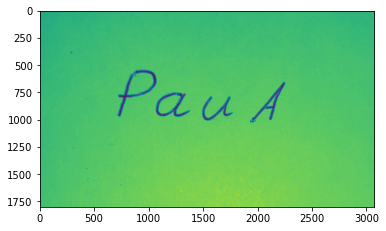
\includegraphics[scale=0.4] {images/before.png}}
\caption{Vaizdas prieš apdorojimą.}
\label{fig2}
\end{figure}

\begin{figure}[!h] % įterpti čia
\centerline{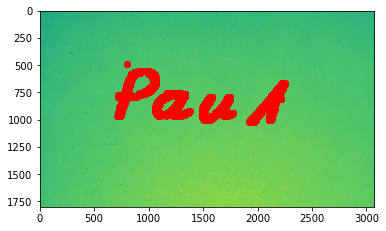
\includegraphics[scale=0.4] {images/after.png}}
\caption{Rastos kraštinės.}
\label{fig3}
\end{figure}

\par
Radus kraštines ir taikant sąlygą, kad vaizde nėra daug pašalinių objektų galima
aproksimuoti Y ašies padėtį, ties kuria yra parašytas tekstas, apskaičiuojant rastų kraštinių
taškų Y koordinates. Rezultatas pateiktas pav. ~\ref{fig4}.

\begin{figure}[!h] % įterpti čia
\centerline{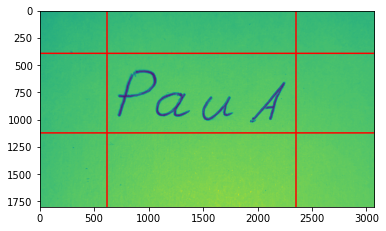
\includegraphics[scale=0.4] {images/aprox.png}}
\caption{Y ašies radimas.}
\label{fig4}
\end{figure}

\par
Radus teksto kraštines yra naudojamas slenkančio lango algoritmas: einama
pro paveikslėlio pikselius ir didinant imamo vaizdo plotis ir vaizdo variantai yra
 siunčiami vaizdai pro
tinklus. Jeigu didinant vaizdo plotį tikimybė sumažėja arba spėjama jog yra kitas
objektas, tada yra ieškoma kitos raidės.

\section{Duomenys}

Sužymėtų duomenų, kurių reikia norint išmokyti modelį, internete nėra, todėl
jie buvo renkami ranka. Ant lapo buvo surašomos raidės ir visas lapas buvo
nufotografuojamas. Gautos fotografijos buvo apdorojamos duomenų žymėjimo programa,
kuri kaip rezultatą eksportavo JSON formato failą su kiekvienos raidės pozicija
nuotraukoje. Pagal gautą JSON failą kiekviena raidė buvo eksportuota į atskirą JPG
failą ir atitinkamai apdorota: naudojant nearest neighbour metodą sumažinta iki
64x64 dydžio ir panaikintas RGB kanalas.

\section{Rezultatai}

Parašyta programa gali aptikti 6 išmoktas raides: A, a, B, C, P, u vidutiniškai su
85\% atspėjimo tikimybe. Raides A, B, C aptinka su 82\% procentų tikimybę, raides a, P, u
su 92\% tikimybe. Padarytą sistemą galima plėsti nemodifikuojant esamo kodo:
užtenka sukurti naują duomenų rinkinį pagal tam tikrą formatą ir ištreniruoti naują
3 elementų aptikimo tinklą. Kadangi programoje naudojama daug skirtingų tinklų ir kiekvienas
jų atskiria tik 3 elementus, plečiant programą, nebereikia apmokyti visos sistemos iš naujo,
užtenka tik pridėti naują tinklą, programa jį automatiškai aptinka ir pradeda naudoti.
Naujam 3 raidžių poaibiui apmokyti reikia vidutiniškai 50 nuotraukų kiekvienai raidei ir
norint pasiekti 85\% tikslumą vidutiniškai užtenka 300 epochų. Naudojant Google Colab
platformą tai vidutiniškai užtrunka apie 10 minučių. Naudojant daug neuroninių tinklų
taip pat išspręsta didelio RAM naudojimo problema: pagal esamus resursus galima
apskaičiuoti kiek vienu momentu galima pakrauti tinklų ir pakrauti tik tam tikrą jų
kiekį.
\par
Dabartinei programos realizacijai trūksta geresnio radžių sričių radimo algoritmo.
Šiuo metu programa aptinka daugiau raidžių nuotraukoje, negul jų yra. Pateikus
programai ~\ref{fig2} pav., programa vietoj rastų raidžių 'PauA', aptinka 'aPAPAPa'.
Programos realizacijoje taip pat trūksta ir modifikuoto SGD algoritmo implementacijos pav. 1. Tikėtina, jog ši modifikacija galėtų pagerinti
tinklo tikslumą.

\printbibliography

\section{Šaltiniai}
\par
[1] Stochastic batch size for adaptive regularization in deep network optimization. Kensuke Nakamura and Stefano Soatto and Byung-Woo Hong. 

\end{document}

